\documentclass[12pt,a4paper]{article}
\usepackage[polish]{babel}
\usepackage{fontspec}
\usepackage[margin=2.5cm]{geometry}
\usepackage{graphicx}
\usepackage{booktabs}
\usepackage{array}
\usepackage{amsmath}
\usepackage{float}
\usepackage{caption}
\usepackage{xurl}
\usepackage[hidelinks]{hyperref}
\usepackage{indentfirst}

\setlength{\parskip}{0.4em}
\sloppy
\setlength{\emergencystretch}{3em}
\renewcommand{\arraystretch}{1.25}
\captionsetup{font=small}
\usepackage{etoolbox}
\AtBeginEnvironment{table}{\small}

% UZUPEŁNIĆ: prowadzący
\newcommand{\autor}{Adam Korwin}
\newcommand{\prowadzacy}{mgr inż. Paweł Tama}

\newcommand{\zrzut}[3][0.95]{%
  \begin{figure}[H]\centering
  \includegraphics[width=#1\textwidth]{#2}
  \caption{#3}\end{figure}}

\begin{document}

\begin{titlepage}
\centering
\vspace*{1cm}

\includegraphics[width=0.28\textwidth]{img/pwr_logo.png}\\[0.4cm]
{\large Politechnika Wrocławska}\\[2.5cm]
\rule{\textwidth}{0.4pt}\\[0.6cm]
{\Huge\scshape Technologie sieciowe}\\[0.5cm]
{\Large\scshape Sprawozdanie z laboratorium nr 1}\\[0.3cm]
{\large Szacowanie pasma}\\[0.3cm]
\rule{\textwidth}{0.4pt}\\[2cm]
{\large\itshape Autor:}\\[0.2cm]
{\large \autor, 284455}\\[1.2cm]
{\large Prowadzący:}\\[0.2cm]
{\large \prowadzacy}\\
\vfill
{\large Wrocław, 16.10.2026}
\end{titlepage}

\tableofcontents
\newpage

\section{Cel ćwiczenia}

Celem ćwiczenia było zmierzenie, ile pasma zużywają typowe usługi internetowe, a następnie
wykorzystanie tych pomiarów do oszacowania przepustowości łącza dla przykładowej firmy i wybrania
dla niej konkretnej oferty dostępnej na rynku. Ruch był przechwytywany programem Wireshark 4.6.9
(dumpcap) na komputerze MacBook z procesorem Apple M4, podłączonym do sieci przez Wi\nobreakdash-Fi (interfejs \texttt{en0}).

\section{Założenia dotyczące firmy}

Numer indeksu kończy się cyfrą 5, więc obowiązuje zestaw danych nr 5:

\begin{table}[H]\centering
\begin{tabular}{cccccc}
\toprule
$X_1$ & $X_2$ & $X_3$ & $X_4$ & $X_5$ & $X_6$ \\
\midrule
25 osób & 30\,\% & 2 stacje & 2 razy/tydz. & 2 stacje & 16 GB \\
\bottomrule
\end{tabular}
\caption{Zestaw danych wejściowych nr 5}
\end{table}

Firma \emph{Mostware sp. z o.o.} to niewielki software house mieszczący się przy
ul.~Generała Romualda Traugutta 45, 50-416 Wrocław. Pracuje w niej 25 osób. Każdy pracownik
przez 30\,\% czasu pracy przegląda strony WWW. Na dwóch stanowiskach przez cały dzień gra radio
internetowe, a na jednym działa streaming wideo (ekran w recepcji). Do komunikacji wszyscy używają
Discorda, telefonów VoIP oraz poczty Gmail obsługiwanej przez przeglądarkę. Dwa razy w tygodniu
odbywają się dwugodzinne wideokonferencje z klientem, w których uczestniczą dwie stacje.
Administrator pobiera przez FTP aktualizacje i obrazy systemów, raz w tygodniu wysyła pełną kopię
bazy danych (16 GB) na zdalny serwer, a codziennie kopię przyrostową o rozmiarze 1/5 bazy, czyli 3,2 GB.
Firma pracuje od 9:00 do 17:00, co daje 8 godzin dziennie.

Zgodnie z sugestią z instrukcji pracownicy zostali podzieleni na grupy, które korzystają z sieci
z różną intensywnością:

\begin{table}[H]\centering
\begin{tabular}{>{\raggedright}p{4.2cm}cccc}
\toprule
Grupa & Liczba osób & Poczta & Komunikator & VoIP \\
 & & [\% czasu] & [\% czasu] & [h/dzień] \\
\midrule
A: zarząd i handlowcy & 4 & 20 & 10 & 3 \\
B: programiści i graficy & 15 & 10 & 15 & 1 \\
C: dział techniczny i admin & 6 & 5 & 20 & 0,5 \\
\bottomrule
\end{tabular}
\caption{Podział pracowników na grupy}
\end{table}

\section{Przebieg ćwiczenia}

\subsection{Sposób generowania ruchu}

Każda usługa była nagrywana w osobnym pliku. Na początku dla każdego pliku sprawdzałem w
Wiresharku adres komputera (10.182.42.126 w dniu 15.10.2026 dla WWW, poczty, komunikatora i radia oraz 10.23.41.207
w dniu 16.10.2026 dla FTP, wideokonferencji i kopii zapasowej) i na jego podstawie rozdzielałem ruch wysyłany (\texttt{ip.src})
od pobieranego (\texttt{ip.dst}).

\begin{table}[H]\centering
\begin{tabular}{>{\raggedright}p{2.6cm}>{\raggedright}p{3.2cm}>{\raggedright\arraybackslash}p{6.2cm}c}
\toprule
Usługa & Program / serwis & Co było robione & Czas \\
\midrule
WWW & przeglądarka & przeglądanie kilku serwisów (m.in. lego.com, zero.pl, kursy LangChain Academy) & 709,7 s \\
Poczta & Gmail w przeglądarce & otwieranie skrzynki, czytanie i wysyłanie wiadomości & 165,9 s \\
Komunikator & Discord (aplikacja) & czat z obrazkami i próba rozmowy głosowej & 231,9 s \\
Radio & radiozet.pl & słuchanie Radia ZET w odtwarzaczu na stronie & 739,2 s \\
FTP & curl & pobieranie obrazu Debian 13.7 z ftp.icm.edu.pl, wysłanie pliku 30 MB na ftp.dlptest.com & 148,6 s \\
Wideo\-kon\-fe\-ren\-cja & Google Meet & spotkanie na laptopie z drugim uczestnikiem na telefonie, kamera i mikrofon włączone & 671,8 s \\
Kopia zapasowa & curl & wysłanie 500 MB losowych danych w 5 częściach po 100 MB na serwer speed.\-cloudflare.\-com & 90,8 s \\
\bottomrule
\end{tabular}
\caption{Opis sposobów generowania ruchu}
\end{table}

W tle na komputerze cały czas działał Claude Code, który komunikuje się z serwerem 160.79.104.10.
Ten ruch nie należy do żadnej z badanych usług, więc wykluczyłem go z filtrów.

Ilości danych podaję w jednostkach dziesiętnych (1 MB = $10^6$ B), a natężenie ruchu liczę jako
\[
R = \frac{8 \cdot B}{T} \quad [\text{b/s}],
\]
gdzie $B$ to liczba bajtów (całe ramki, razem z nagłówkami), a $T$ to czas pomiaru w sekundach.

\subsection{WWW}

Filtr dla ruchu wysyłanego miał postać
\texttt{ip.src == 10.182.42.126 \&\& (tcp.port in \{80, 443\} || udp.port == 443)},
a dla pobieranego analogicznie z \texttt{ip.dst}. Port UDP 443 jest potrzebny, bo duża część
stron korzysta już z HTTP/3 (QUIC). Widać to w hierarchii protokołów: QUIC przenosi ponad połowę
pobranych bajtów, a zwykłe HTTP bez szyfrowania to tylko 14 pakietów.

Zrzuty poniżej zostały zrobione z tym filtrem, czyli jeszcze bez wykluczenia ruchu Claude Code.
Pokazują one 14\,173\,960 B wysłanych (58\,453 pakiety) i 140\,157\,510 B pobranych
(127\,411 pakietów). Do obliczeń użyłem filtra uzupełnionego o
\texttt{\&\& !(ip.addr == 160.79.104.10)}, po którym zostaje 13\,911\,999 B wysłanych
i 139\,813\,165 B pobranych. Różnica to ok. 1,8\,\% w górę i 0,2\,\% w dół.

\zrzut{img/www_wlasciwosci.png}{Właściwości pliku www.pcapng (kolumna Displayed dla filtru ruchu wysyłanego)}
\zrzut{img/www_hier_dst.png}{Hierarchia protokołów, ruch pobierany (WWW)}
\zrzut{img/www_hier_src.png}{Hierarchia protokołów, ruch wysyłany (WWW)}
\zrzut{img/www_io.png}{Wykres I/O dla ruchu WWW, przedziały 1 s}

\begin{table}[H]\centering
\begin{tabular}{ccccc}
\toprule
\shortstack{Razem\\{}[MB]} & \shortstack{Pobrane\\{}[MB]} & \shortstack{Wysłane\\{}[MB]} & \shortstack{Down\\{}[Mb/s]} & \shortstack{Up\\{}[Mb/s]} \\
\midrule
153,73 & 139,81 & 13,91 & 1,576 & 0,157 \\
\bottomrule
\end{tabular}
\caption{Wyniki dla WWW}
\end{table}

\[
R_{\text{down}} = \frac{8 \cdot 139\,813\,165}{709{,}7} \approx 1\,576\ \text{kb/s}, \qquad
R_{\text{up}} = \frac{8 \cdot 13\,911\,999}{709{,}7} \approx 157\ \text{kb/s}
\]

Ruch WWW jest bardzo nierówny. Przez większość czasu łącze stoi prawie puste (czytanie strony),
a po kliknięciu w link pojawia się krótki skok do kilkunastu Mb/s. Najwyższa wartość w ciągu
jednej sekundy wyniosła 19,8 Mb/s, czyli ponad 12 razy więcej niż średnia.

\subsection{Poczta elektroniczna}

Pierwsza próba filtrowania po portach pocztowych
(\texttt{tcp.port in \{25, 465, 587, 143, 993, 110, 995\}}) dała tylko 5 pakietów. Wynika to
z tego, że Gmail obsługiwany w przeglądarce nie używa SMTP ani IMAP, tylko zwykłego HTTPS/QUIC.
Dlatego dla poczty zastosowałem ten sam filtr co dla WWW. W czasie nagrywania przeglądarka miała
otwartą tylko skrzynkę Gmail, a jedyne obce połączenie (meet.google.com, 142.251.154.5) wykluczyłem:
\texttt{(tcp.port in \{80, 443\} || udp.port == 443) \&\& !(ip.addr in \{160.79.104.10, 142.251.154.5\})}.
Zrzuty zostały zrobione z samym filtrem portów, bez tego wykluczenia, i pokazują
3\,138\,615 B wysłanych (10\,858 pakietów) oraz 20\,144\,871 B pobranych. Po wykluczeniu
zostaje 2\,975\,390 B wysłanych i 18\,923\,813 B pobranych i te wartości są w tabeli.

\zrzut{img/poczta_wlasciwosci.png}{Właściwości pliku poczta.pcapng}
\zrzut[0.8]{img/poczta_porty.png}{Filtr po portach SMTP/IMAP/POP3 daje tylko 5 pakietów}
\zrzut{img/poczta_hier_src.png}{Hierarchia protokołów dla ruchu wysyłanego (poczta)}
\zrzut{img/poczta_io.png}{Wykres I/O dla poczty}

\begin{table}[H]\centering
\begin{tabular}{ccccc}
\toprule
\shortstack{Razem\\{}[MB]} & \shortstack{Pobrane\\{}[MB]} & \shortstack{Wysłane\\{}[MB]} & \shortstack{Down\\{}[Mb/s]} & \shortstack{Up\\{}[Mb/s]} \\
\midrule
21,90 & 18,92 & 2,98 & 0,913 & 0,144 \\
\bottomrule
\end{tabular}
\caption{Wyniki dla poczty}
\end{table}

\[
R_{\text{down}} = \frac{8 \cdot 18\,923\,813}{165{,}9} \approx 913\ \text{kb/s}, \qquad
R_{\text{up}} = \frac{8 \cdot 2\,975\,390}{165{,}9} \approx 144\ \text{kb/s}
\]

Na wykresie widać dwa okresy większego ruchu. Pierwsze 70 sekund to ładowanie samej aplikacji
Gmail i otwieranie kolejnych wiadomości, a krótkie skoki do ok. 8,7 Mb/s w okolicy 120 s to otwieranie wiadomości z większą zawartością.
Średnia jest zawyżona przez to, że webowy klient poczty przy starcie ściąga kilka megabajtów
skryptów. Przy dłuższym korzystaniu ze skrzynki ruch byłby niższy.

\subsection{Komunikator (Discord)}

Na początku użyłem filtra
\texttt{ip.src == 10.182.42.126 \&\& (udp \&\& !(udp.port in \{53, 443, 5353\}))},
który miał wyciągnąć sam ruch głosowy. Okazało się jednak, że zostają po nim tylko 362 pakiety
wysłane i 637 odebranych (połączenie z 104.29.148.109, port 19315), czyli ok. 1,8 kb/s w górę
i 2,6 kb/s w dół. To około 3 pakiety na sekundę, podczas gdy kodek Opus przy mówieniu wysyła
50 pakietów na sekundę. Oznacza to, że w czasie pomiaru w rozmowie praktycznie nikt nie mówił,
a przez łącze szły tylko pakiety podtrzymujące (STUN, SRTCP). Ten wynik nie nadaje się do
szacowania ruchu VoIP, więc rozmowy głosowe w obliczeniach policzyłem teoretycznie (punkt~\ref{sec:obliczenia}).

Pełny ruch Discorda, razem z czatem i ładowaniem obrazków, wyciągnąłem filtrem na adresy
Discorda (Cloudflare, 162.159.0.0/16) i serwer głosowy:
\texttt{ip.addr == 162.159.0.0/16 || ip.addr == 104.29.148.109}.

\zrzut{img/discord_wlasciwosci.png}{Właściwości pliku discord.pcapng (Displayed dla filtru UDP)}
\zrzut{img/discord_hier_src.png}{Hierarchia protokołów, wysyłany ruch UDP Discorda}
\zrzut{img/discord_hier_dst.png}{Hierarchia protokołów, odbierany ruch UDP Discorda}
\zrzut{img/discord_io.png}{Wykres I/O dla Discorda}

\begin{table}[H]\centering
\begin{tabular}{>{\raggedright}p{3.2cm}ccccc}
\toprule
Zakres & \shortstack{Razem\\{}[MB]} & \shortstack{Pobrane\\{}[MB]} & \shortstack{Wysłane\\{}[MB]} & \shortstack{Down\\{}[kb/s]} & \shortstack{Up\\{}[kb/s]} \\
\midrule
cały Discord & 12,90 & 11,79 & 1,11 & 406,7 & 38,4 \\
tylko UDP (głos) & 0,127 & 0,076 & 0,051 & 2,6 & 1,8 \\
\bottomrule
\end{tabular}
\caption{Wyniki dla Discorda}
\end{table}

\[
R_{\text{down}} = \frac{8 \cdot 11\,788\,741}{231{,}9} \approx 407\ \text{kb/s}, \qquad
R_{\text{up}} = \frac{8 \cdot 1\,111\,678}{231{,}9} \approx 38\ \text{kb/s}
\]

Prawie cały ruch przypada na pierwsze 60 sekund, kiedy aplikacja ładowała kanały i obrazki
(skoki do 10 Mb/s). Później sam czat generuje bardzo mało danych, pojedyncze kilobajty na sekundę.

\subsection{Radio internetowe}

Pierwszy filtr, którego użyłem, obejmował cały ruch HTTPS komputera z wyłączeniem serwera
Claude Code. Daje on średnio 766 kb/s, co jest wartością zdecydowanie za dużą jak na radio.
Po sprawdzeniu w statystyce \emph{Conversations} i w zapytaniach DNS okazało się, że strona
radiozet.pl ładuje dużo reklam (criteo, rubiconproject, adtelligent) i odtwarza reklamy wideo
z serwerów Google. Sam strumień audio pochodzi z jednego serwera:
\texttt{25443.live.streamtheworld.com} (107.155.103.139). Dlatego właściwy filtr dla radia to
\texttt{ip.addr == 107.155.103.139}.

\zrzut{img/radio_wlasciwosci.png}{Właściwości pliku radio.pcapng (Displayed dla filtru całej strony)}
\zrzut{img/radio_hier.png}{Hierarchia protokołów dla całego ruchu strony radiozet.pl}
\zrzut{img/radio_io.png}{Wykres I/O dla całej strony radiozet.pl}

\begin{figure}[H]\centering
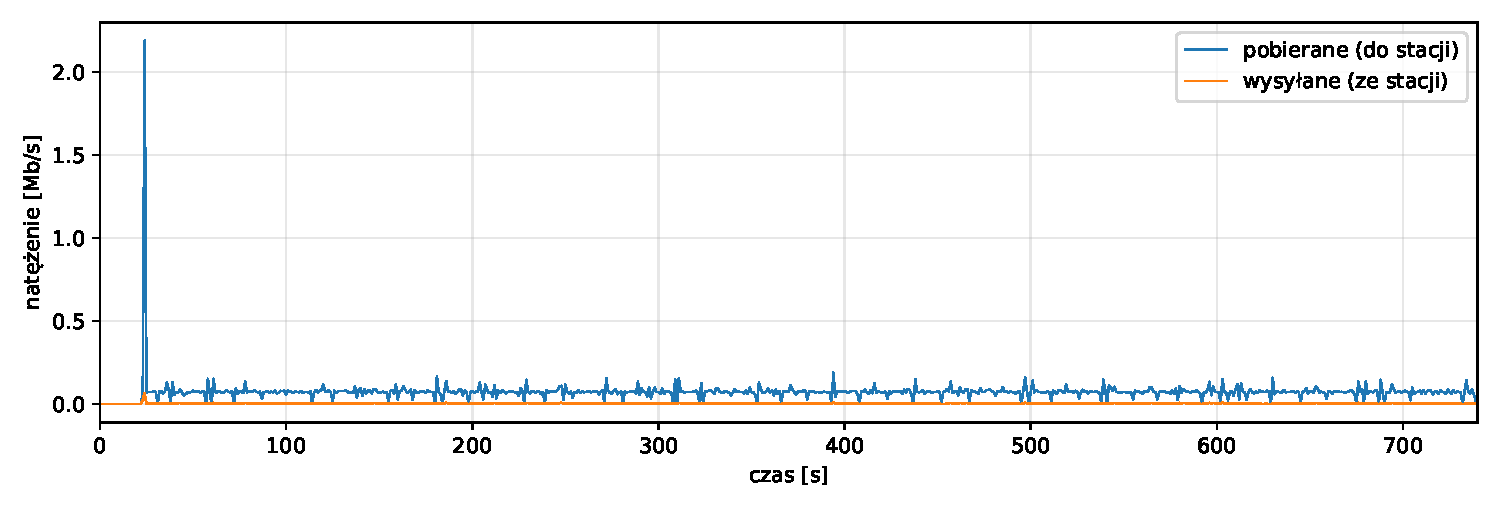
\includegraphics[width=\textwidth]{wykresy/radio.pdf}
\caption{Natężenie ruchu dla samego strumienia audio (filtr \texttt{ip.addr == 107.155.103.139}), przedziały 1 s}
\end{figure}

\begin{table}[H]\centering
\begin{tabular}{>{\raggedright}p{3.2cm}ccccc}
\toprule
Zakres & \shortstack{Razem\\{}[MB]} & \shortstack{Pobrane\\{}[MB]} & \shortstack{Wysłane\\{}[MB]} & \shortstack{Down\\{}[kb/s]} & \shortstack{Up\\{}[kb/s]} \\
\midrule
strumień audio & 7,12 & 6,79 & 0,34 & 73,4 & 3,6 \\
cała strona & 70,82 & 55,58 & 15,25 & 601,5 & 165,0 \\
\bottomrule
\end{tabular}
\caption{Wyniki dla radia internetowego}
\end{table}

\[
R_{\text{down}} = \frac{8 \cdot 6\,785\,671}{739{,}2} \approx 73{,}4\ \text{kb/s}, \qquad
R_{\text{up}} = \frac{8 \cdot 335\,874}{739{,}2} \approx 3{,}6\ \text{kb/s}
\]

Strumień audio ma bardzo równy przebieg. Na początku jest jeden skok do 2,2 Mb/s, kiedy
odtwarzacz wypełnia bufor, a potem ruch utrzymuje się na poziomie ok. 70 kb/s, co odpowiada
typowemu strumieniowi audio 64 kb/s z narzutem nagłówków. Do obliczeń przyjąłem wartość dla samego
strumienia, bo na stanowiskach w firmie radio można słuchać w zwykłym odtwarzaczu, bez reklam
na stronie.

\subsection{FTP}

Ruch FTP nagrałem osobno, 16.10.2026. Pobierany był obraz \texttt{debian-13.7.0-amd64-netinst.iso}
z serwera ftp.icm.edu.pl (193.219.28.2, logowanie anonimowe, tryb pasywny EPSV). Pobieranie
przerwałem po 120 sekundach, po ściągnięciu 652 MB. Następnie na testowy serwer ftp.dlptest.com
(44.241.66.173) został wysłany plik z losową zawartością o rozmiarze 30 MB, który miał symulować
kopię zapasową. Po teście plik został usunięty z serwera. Filtry:
\texttt{ip.addr == 193.219.28.2} dla pobierania i \texttt{ip.addr == 44.241.66.173} dla wysyłania.
W hierarchii protokołów dla ruchu pobieranego widać, że 450\,636 pakietów należy do kanału
danych (FTP Data), a tylko 15 to odpowiedzi serwera na kanale sterującym (FTP).

\zrzut{img/ftp_wlasciwosci.png}{Właściwości pliku ftp.pcapng (Displayed dla ruchu pobieranego z ftp.icm.edu.pl)}
\zrzut{img/ftp_hier_dst.png}{Hierarchia protokołów, ruch pobierany przez FTP}

Wykres I/O z Wiresharka dla tego pliku (825 MB) rysował się niepełny, część transferu
była na nim pokazana jako zero. Wykresy natężenia poniżej zostały więc wyliczone z tego samego
pliku programem tshark, w przedziałach 1 s.

\begin{figure}[H]\centering
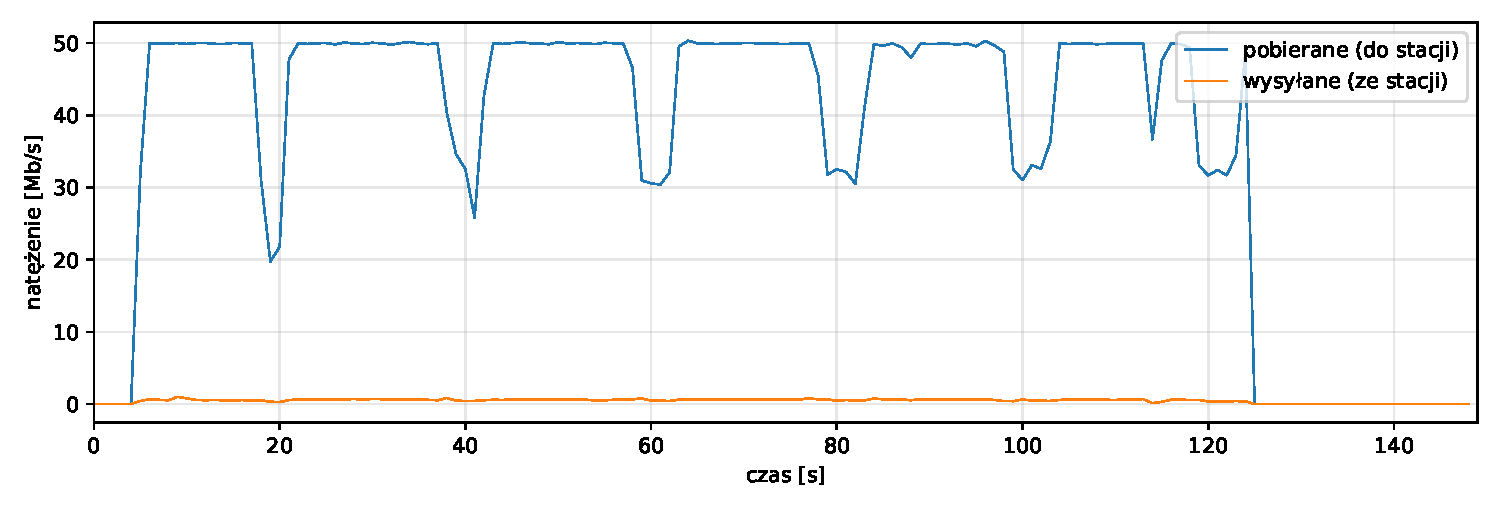
\includegraphics[width=\textwidth]{wykresy/ftp_down.pdf}
\caption{Natężenie ruchu przy pobieraniu przez FTP (ftp.icm.edu.pl)}
\end{figure}

\begin{figure}[H]\centering
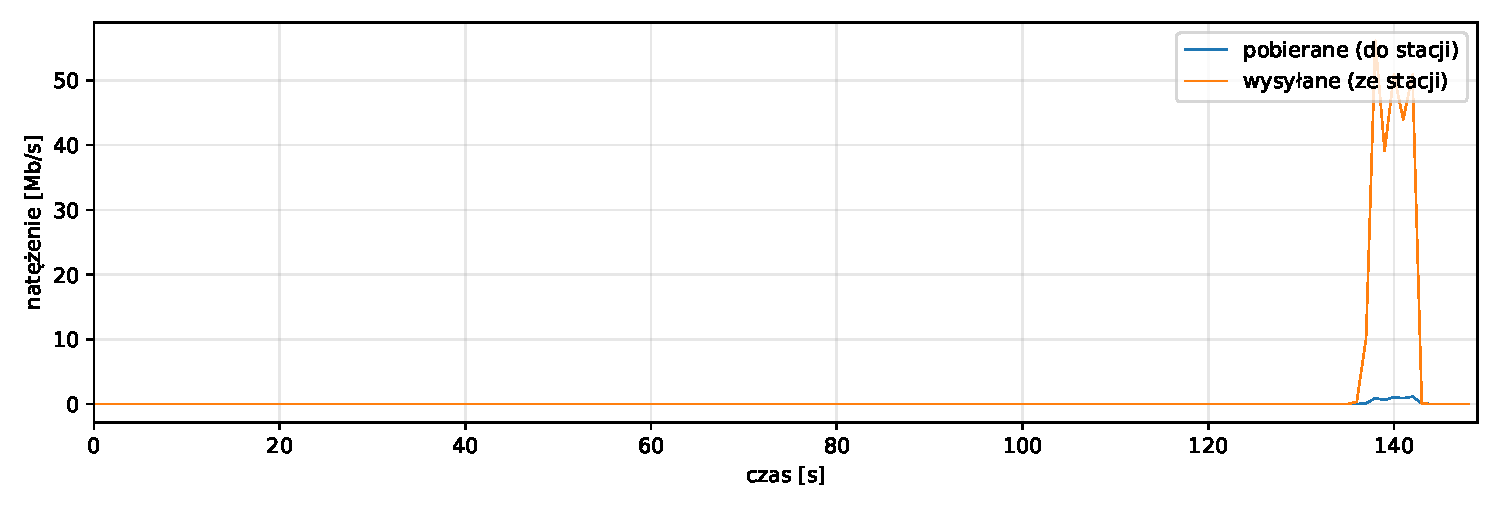
\includegraphics[width=\textwidth]{wykresy/ftp_up.pdf}
\caption{Natężenie ruchu przy wysyłaniu przez FTP (ftp.dlptest.com)}
\end{figure}

\begin{table}[H]\centering
\begin{tabular}{>{\raggedright}p{2.2cm}cccccc}
\toprule
Kierunek & \shortstack{Czas\\{}[s]} & \shortstack{Razem\\{}[MB]} & \shortstack{Pobrane\\{}[MB]} & \shortstack{Wysłane\\{}[MB]} & \shortstack{Down\\{}[Mb/s]} & \shortstack{Up\\{}[Mb/s]} \\
\midrule
pobieranie & 120,2 & 691,90 & 683,16 & 8,74 & 45,47 & 0,58 \\
wysyłanie & 8,9 & 32,07 & 0,62 & 31,45 & 0,55 & 28,27 \\
\bottomrule
\end{tabular}
\caption{Wyniki dla FTP (czas liczony od pierwszego do ostatniego pakietu transferu)}
\end{table}

\[
R_{\text{down}} = \frac{8 \cdot 683\,162\,190}{120{,}2} \approx 45{,}5\ \text{Mb/s}, \qquad
R_{\text{up}} = \frac{8 \cdot 31\,451\,890}{8{,}9} \approx 28{,}3\ \text{Mb/s}
\]

FTP zachowuje się zupełnie inaczej niż pozostałe usługi. Nie ma swojej stałej przepływności,
tylko zajmuje tyle pasma, ile jest dostępne. Wykres pobierania jest płaski na poziomie ok. 50 Mb/s,
co oznacza ograniczenie gdzieś na trasie. Bez osobnego testu prędkości nie da się rozstrzygnąć,
czy był to limit serwera, czy sieci Wi\nobreakdash-Fi, tym bardziej że tego samego dnia wysyłanie
osiągało chwilowo 82,6 Mb/s. Spadki do ok. 30 Mb/s najpewniej wynikają z innego ruchu na tym
samym łączu, bo w czasie pomiaru w przeglądarce było odtwarzane wideo. W kierunku
przeciwnym do transferu płyną tylko potwierdzenia TCP, które stanowią ok. 1,3\,\% ruchu przy
pobieraniu i ok. 2\,\% przy wysyłaniu.

\subsection{Wideokonferencja (Google Meet)}

Wideokonferencję nagrałem 16.10.2026. Spotkanie w Google Meet było założone na laptopie,
a drugi uczestnik dołączył z telefonu. Na obu urządzeniach
działała kamera i mikrofon. Meet przesyła obraz i dźwięk po UDP do serwerów mediów Google,
dlatego filtr dla ruchu wysyłanego miał postać
\texttt{ip.src == 10.23.41.207 \&\& (udp.port in \{3478, 19302..19309\} || ip.addr == 74.125.250.0/24 || ip.addr == 142.250.82.0/24)},
a dla pobieranego analogicznie z \texttt{ip.dst}. W statystyce \emph{Conversations} widać, że cały
ruch spotkania szedł jednym połączeniem UDP z serwerem 142.250.82.212 na porcie 3478. W hierarchii
protokołów prawie wszystko trafia do kategorii \emph{Data}, bo media są zaszyfrowane (SRTP)
i Wireshark nie rozpoznaje ich zawartości. Rozpoznane zostały tylko pakiety kontrolne STUN, RTCP
i DTLS. Pakiety oznaczone jako \emph{Malformed} przy RTCP (ok. 7,7\,\% wysłanych) to zaszyfrowane
raporty SRTCP, których zawartości Wireshark nie potrafi poprawnie zdekodować, a nie błędy transmisji.

\zrzut{img/meet_wlasciwosci.png}{Właściwości pliku google meets.pcapng (cały plik, bez filtra)}
\zrzut{img/meet_hier_src.png}{Hierarchia protokołów, ruch wysyłany (Google Meet)}
\zrzut{img/meet_hier_dst.png}{Hierarchia protokołów, ruch pobierany (Google Meet)}
\zrzut{img/meet_io.png}{Wykres I/O dla Google Meet (niebieski: wysyłane, brązowy: pobierane)}

\begin{table}[H]\centering
\begin{tabular}{>{\raggedright}p{3.4cm}ccccc}
\toprule
Zakres & \shortstack{Razem\\{}[MB]} & \shortstack{Pobrane\\{}[MB]} & \shortstack{Wysłane\\{}[MB]} & \shortstack{Down\\{}[Mb/s]} & \shortstack{Up\\{}[Mb/s]} \\
\midrule
całe połączenie (646,3 s) & 223,07 & 116,88 & 106,19 & 1,447 & 1,314 \\
pełna rozmowa (200--650 s) & 196,43 & 103,10 & 93,33 & 1,833 & 1,659 \\
\bottomrule
\end{tabular}
\caption{Wyniki dla wideokonferencji}
\end{table}

\[
R_{\text{down}} = \frac{8 \cdot 116\,878\,355}{646{,}3} \approx 1{,}447\ \text{Mb/s}, \qquad
R_{\text{up}} = \frac{8 \cdot 106\,191\,393}{646{,}3} \approx 1{,}314\ \text{Mb/s}
\]

Przez pierwsze ok. 150 sekund ruchu Meet było mało, bo w tym czasie ładowała się strona i dołączał
drugi uczestnik. Wysokie skoki do 22--31 Mb/s widoczne na wykresie I/O w tym okresie należą do
krzywej \emph{All packets}, czyli do innego ruchu komputera, a nie do spotkania. Pozostałe pozycje
\emph{Filtered packets} w legendzie to wyłączone linie z domyślnej konfiguracji Wiresharka. Od ok. 200 s rozmowa trwała już normalnie. Wysyłanie jest wtedy bardzo równe,
cały czas ok. 1,66 Mb/s, bo kamera laptopa nadaje obraz o stałej jakości. Pobieranie zmienia się
od ok. 0,7 do 2,5 Mb/s, ponieważ Meet dopasowuje jakość obrazu z telefonu do warunków w sieci. Pojedynczy skok do 3,7 Mb/s pojawił się przy zmianie jakości. Do obliczeń przyjąłem
wartości z pełnej rozmowy (200 do 650 s), bo średnia z całego pliku zaniża wynik przez okres
dołączania. Ruch jest prawie symetryczny, stosunek pobierania do wysyłania wynosi ok. 1,1.

\subsection{Kopia zapasowa}

Wysłanie prawdziwej kopii 16 GB nie było możliwe, więc przesyłanie kopii zasymulowałem
mniejszym plikiem. Na serwer testu prędkości Cloudflare (speed.cloudflare.com, adresy
172.66.0.218 i 162.159.140.220) zostało wysłane pięć razy po 100 MB losowych danych przez HTTPS,
jedna część po drugiej, tak jak program do kopii wysyła kolejne paczki. Losowe dane nie dają się
skompresować, więc przypominają zaszyfrowane archiwum bazy. Filtr:
\texttt{ip.addr in \{172.66.0.218, 162.159.140.220\}}. Nagrywanie odbywało się z filtrem
przechwytywania na te dwa adresy, więc w pliku nie ma innego ruchu.

\zrzut{img/backup_wlasciwosci.png}{Właściwości pliku backup.pcapng (Displayed dla ruchu wysyłanego)}
\zrzut{img/backup_hier_src.png}{Hierarchia protokołów, ruch wysyłany przy kopii zapasowej}

W hierarchii cały ruch to TCP z TLS. Rekordów TLS jest tylko 30\,545, bo jeden rekord zajmuje
kilka segmentów TCP, a Wireshark przypisuje go do ostatniego z nich. Wykres natężenia, tak jak dla
FTP, został wyliczony programem tshark, bo wykres I/O w Wiresharku pokazywał tylko końcową część
wysyłania.

\begin{figure}[H]\centering
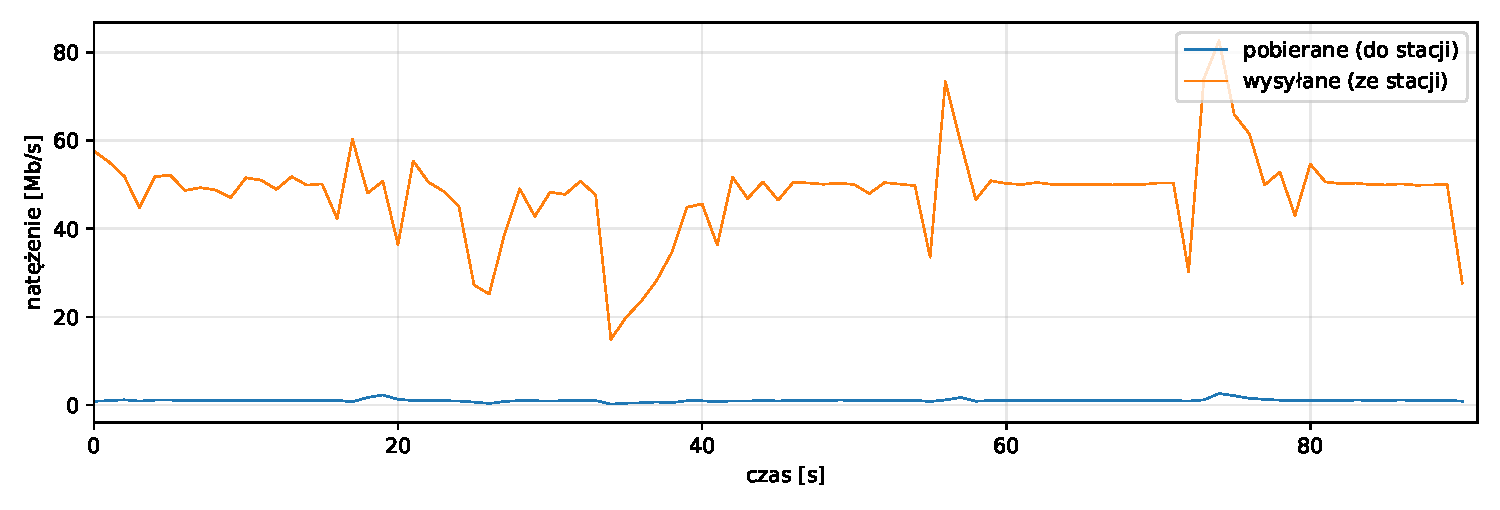
\includegraphics[width=\textwidth]{wykresy/backup.pdf}
\caption{Natężenie ruchu przy wysyłaniu kopii zapasowej (500 MB w 5 częściach)}
\end{figure}

\begin{table}[H]\centering
\begin{tabular}{ccccccc}
\toprule
\shortstack{Czas\\{}[s]} & \shortstack{Razem\\{}[MB]} & \shortstack{Pobrane\\{}[MB]} & \shortstack{Wysłane\\{}[MB]} & \shortstack{Down\\{}[Mb/s]} & \shortstack{Up\\{}[Mb/s]} & \shortstack{Max up\\{}[Mb/s]} \\
\midrule
90,8 & 558,98 & 11,82 & 547,16 & 1,04 & 48,21 & 82,6 \\
\bottomrule
\end{tabular}
\caption{Wyniki dla kopii zapasowej}
\end{table}

\[
R_{\text{up}} = \frac{8 \cdot 547\,161\,623}{90{,}8} \approx 48{,}2\ \text{Mb/s}
\]

Kolejne części były wysyłane jedna po drugiej, więc przebieg jest prawie ciągły, na poziomie
ok. 50 Mb/s. Widać tylko kilka krótkich spadków, m.in. przy zestawianiu nowego połączenia.
Ważniejsze od samej prędkości jest to, ile danych naprawdę przechodzi przez łącze. Wysłane było
500\,000\,000 B danych, a ramek wyszło 547\,161\,623 B:
\[
k = \frac{547\,161\,623}{500\,000\,000} \approx 1{,}094
\]
Te 9,4\,\% nie są jednak samym narzutem nagłówków. Filtr \texttt{tcp.analysis.retransmission}
pokazuje 15\,614 retransmisji TCP o łącznej wielkości 22\,663\,216 B (4,1\,\% wysłanych bajtów),
czyli strat na Wi\nobreakdash-Fi. Po ich odjęciu zostaje
\[
k_{\text{prot}} = \frac{547\,161\,623 - 22\,663\,216}{500\,000\,000} \approx 1{,}049,
\]
więc nagłówki Ethernet, IP, TCP, TLS i HTTP to ok. 4,9\,\%, a retransmisje drugie tyle.
W dalszych obliczeniach zostawiam pełne $k = 1{,}094$ jako bezpieczne oszacowanie, bo
łącze w firmie też nie musi być bezstratne. W przeciwną stronę wracają tylko potwierdzenia TCP,
ok. 2,2\,\% wysłanych bajtów.
Przy zmierzonej prędkości 48,2 Mb/s pełna kopia 16 GB i kopia dzienna 3,2 GB wysyłałyby się w czasie
\[
t_{\text{pełna}} = \frac{16 \cdot 10^9 \cdot 1{,}094 \cdot 8}{48{,}2 \cdot 10^6} \approx 2\,905\ \text{s} \approx 48\ \text{min},
\]
\[
t_{\text{dzienna}} = \frac{3{,}2 \cdot 10^9 \cdot 1{,}094 \cdot 8}{48{,}2 \cdot 10^6} \approx 581\ \text{s} \approx 10\ \text{min}.
\]

\subsection{Podsumowanie pomiarów}

\begin{table}[H]\centering
\begin{tabular}{>{\raggedright}p{3.6cm}ccc}
\toprule
Usługa & Down [kb/s] & Up [kb/s] & Stosunek down/up \\
\midrule
WWW & 1\,575,9 & 156,8 & 10,1 \\
Poczta (Gmail) & 912,6 & 143,5 & 6,4 \\
Discord (czat) & 406,7 & 38,4 & 10,6 \\
Radio (strumień) & 73,4 & 3,6 & 20,4 \\
FTP pobieranie & 45\,468 & 582 & 78,1 \\
FTP wysyłanie & 554 & 28\,271 & 0,02 \\
Google Meet (rozmowa) & 1\,833 & 1\,659 & 1,1 \\
Kopia zapasowa & 1\,041 & 48\,208 & 0,02 \\
\bottomrule
\end{tabular}
\caption{Zestawienie zmierzonych natężeń ruchu}
\end{table}

\subsection{Wyliczenie przepustowości łącza}\label{sec:obliczenia}

Dla każdej usługi liczę, ilu użytkowników korzysta z niej jednocześnie w typowej chwili dnia pracy,
i mnożę to przez zmierzone natężenie. Dla usług, których nie mierzyłem albo pomiar okazał się
niewiarygodny, przyjąłem wartości szacunkowe i zaznaczyłem to w tabeli.

\paragraph{WWW.} 25 osób przez 30\,\% czasu, czyli średnio $25 \cdot 0{,}3 = 7{,}5$ osoby naraz:
\[
7{,}5 \cdot 1{,}576 = 11{,}82\ \text{Mb/s (down)}, \qquad 7{,}5 \cdot 0{,}157 = 1{,}18\ \text{Mb/s (up)}
\]

\paragraph{Poczta.} Liczba równoczesnych użytkowników wynika z podziału na grupy:
\[
4 \cdot 0{,}20 + 15 \cdot 0{,}10 + 6 \cdot 0{,}05 = 2{,}6
\]
\[
2{,}6 \cdot 0{,}913 = 2{,}37\ \text{Mb/s (down)}, \qquad 2{,}6 \cdot 0{,}144 = 0{,}37\ \text{Mb/s (up)}
\]

\paragraph{Komunikator.}
\[
4 \cdot 0{,}10 + 15 \cdot 0{,}15 + 6 \cdot 0{,}20 = 3{,}85
\]
\[
3{,}85 \cdot 0{,}407 = 1{,}57\ \text{Mb/s (down)}, \qquad 3{,}85 \cdot 0{,}038 = 0{,}15\ \text{Mb/s (up)}
\]

\paragraph{VoIP.} Przyjąłem kodek G.711 i pakiety co 20 ms, czyli 50 pakietów na sekundę.
Jeden pakiet to 160 B głosu, 12 B nagłówka RTP, 8 B UDP, 20 B IP i 14 B nagłówka Ethernet,
razem 214 B. Pole FCS (4 B) pomijam, bo Wireshark nie liczy go też w pozostałych pomiarach:
\[
R_{\text{VoIP}} = 214 \cdot 8 \cdot 50 = 85{,}6\ \text{kb/s w każdą stronę}
\]
Natężenie ruchu telefonicznego w ciągu 8\nobreakdash-godzinnego dnia:
\[
A = \frac{4 \cdot 3 + 15 \cdot 1 + 6 \cdot 0{,}5}{8} = \frac{30}{8} = 3{,}75\ \text{Erl}
\]
Rozmowy nie rozkładają się równo w czasie, więc liczbę równoczesnych rozmów, którą łącze musi
obsłużyć, policzyłem wzorem Erlanga B dla prawdopodobieństwa blokady 1\,\%:
\[
B(A, N) = \frac{\dfrac{A^N}{N!}}{\displaystyle\sum_{i=0}^{N} \dfrac{A^i}{i!}}, \qquad
B(3{,}75;\ 8) \approx 2{,}3\,\%, \qquad B(3{,}75;\ 9) \approx 0{,}96\,\%
\]
Potrzeba więc $N = 9$ równoczesnych rozmów:
\[
9 \cdot 85{,}6 = 0{,}77\ \text{Mb/s w każdą stronę}
\]

\paragraph{Radio.} Dwie stacje przez cały dzień:
$2 \cdot 73{,}4 = 0{,}15$ Mb/s (down) i $2 \cdot 3{,}6 = 0{,}01$ Mb/s (up).

\paragraph{Streaming wideo.} Nie był mierzony. Przyjąłem 5 Mb/s, co odpowiada zalecanej
przepływności dla wideo 1080p w serwisie YouTube, oraz 0,1 Mb/s w górę na potwierdzenia.

\paragraph{Wideokonferencja.} Dwie stacje, wartości z pełnej rozmowy w Google Meet:
\[
2 \cdot 1{,}833 = 3{,}67\ \text{Mb/s (down)}, \qquad 2 \cdot 1{,}659 = 3{,}32\ \text{Mb/s (up)}
\]
Wideokonferencje są tylko dwa razy w tygodniu, ale łącze musi je obsłużyć w momencie, kiedy trwają,
więc wliczam je do sumy.

\paragraph{FTP (aktualizacje).} Założyłem, że administrator pobiera ok. 3 GB aktualizacji dziennie.
W przeliczeniu na dzień pracy:
\[
\frac{3 \cdot 10^9 \cdot 8}{8 \cdot 3600} = 0{,}83\ \text{Mb/s}
\]
Pomiar pokazał, że FTP i tak zajmie całe wolne pasmo, więc ta wartość nie jest wymaganiem
na szybkość, tylko średnim obciążeniem.

\paragraph{Kopia zapasowa.} Kopie są wysyłane po godzinach pracy, więc nie sumują się z ruchem
dziennym. Pełna kopia 16 GB raz w tygodniu powinna zmieścić się w 4 godzinach (17:00 do 21:00),
a codzienna kopia 3,2 GB w jednej godzinie. Uwzględniam zmierzony narzut $k = 1{,}094$:
\[
R_{\text{pełna}} = \frac{16 \cdot 10^9 \cdot 1{,}094 \cdot 8}{4 \cdot 3600} = 9{,}73\ \text{Mb/s}, \qquad
R_{\text{dzienna}} = \frac{3{,}2 \cdot 10^9 \cdot 1{,}094 \cdot 8}{3600} = 7{,}78\ \text{Mb/s}
\]
W stronę firmy wracają przy tym potwierdzenia, ok. 2,2\,\% tych wartości.

\begin{table}[H]\centering
\begin{tabular}{>{\raggedright}p{3.4cm}c>{\raggedright}p{3.0cm}cc}
\toprule
Usługa & Jednostki & Częstotliwość & \shortstack{Down\\{}[Mb/s]} & \shortstack{Up\\{}[Mb/s]} \\
\midrule
WWW & 25 & 30\,\% czasu & 11,82 & 1,18 \\
Poczta & 25 & wg grup (2,6 os.) & 2,37 & 0,37 \\
Komunikator & 25 & wg grup (3,85 os.) & 1,57 & 0,15 \\
VoIP$^{*}$ & 25 & 9 rozmów (Erlang B) & 0,77 & 0,77 \\
Radio & 2 & cały dzień & 0,15 & 0,01 \\
Streaming wideo$^{*}$ & 1 & cały dzień & 5,00 & 0,10 \\
Wideokonferencja & 2 & 2$\times$2 h/tydz. & 3,67 & 3,32 \\
FTP aktualizacje & 1 & 3 GB/dzień & 0,83 & 0,01 \\
\midrule
\multicolumn{3}{r}{\textbf{Suma w godzinach pracy}} & \textbf{26,18} & \textbf{5,91} \\
\multicolumn{3}{r}{\textbf{Z zapasem 50\,\%}} & \textbf{39,27} & \textbf{8,87} \\
\midrule
Backup pełny & 1 & 1$\times$/tydz., 4 h & 0,21 & 9,73 \\
Backup dzienny & 1 & 1$\times$/dzień, 1 h & 0,17 & 7,78 \\
\bottomrule
\end{tabular}

\vspace{0.2em}
{\small $^{*}$ wartości przyjęte, nie zmierzone}
\caption{Wyliczenie przepustowości łącza dla firmy Mostware}
\end{table}

Zapas 50\,\% dodałem z dwóch powodów. Po pierwsze, policzone wartości są średnie, a pomiary
pokazały, że chwilowe skoki są wielokrotnie wyższe (dla WWW ponad 12 razy). Po drugie, w firmie
mogą pojawić się usługi, których tu nie uwzględniłem, np. aktualizacje systemów na stacjach
roboczych czy synchronizacja plików w chmurze. Firma potrzebuje więc łącza o przepustowości
co najmniej ok. 40 Mb/s w dół i 10 Mb/s w górę. W kierunku do Internetu o wymaganiu decyduje
pełna kopia zapasowa (9,73 Mb/s), a nie ruch w godzinach pracy.

\section{Wybór łącza do Internetu}

Pod adresem firmy dostępne są oferty światłowodowe Orange i Play dla firm. Najtańsze warianty
obu operatorów (do 300 Mb/s) z dużym zapasem pokrywają policzone zapotrzebowanie, więc o wyborze
zdecydowały dodatkowe parametry: prędkość wysyłania, stały adres IP potrzebny do zdalnego
dostępu i kopii zapasowych, a także czas usunięcia awarii.

\begin{table}[H]\centering
\begin{tabular}{>{\raggedright}p{4.4cm}ccc}
\toprule
Oferta (24 mies.) & Down/Up [Mb/s] & Średnia cena netto & Stały IP i SLA \\
\midrule
Orange Światłowód 300 Mb/s & 300 / 50 & 41,26 zł & w Paczce L \\
Orange Światłowód 1 Gb/s & 1000 / 300 & 46,30 zł & w Paczce L \\
Play Światłowód 300 Mb/s & 300 / b.d. & 50,00 zł & brak \\
Play Światłowód 1 Gb/s & 1000 / b.d. & 70,00 zł & tak, SLA 12 h \\
\bottomrule
\end{tabular}
\caption{Porównanie ofert (ceny ze stron operatorów, październik 2026)}
\end{table}

Wybrałem \textbf{Orange Światłowód do 1 Gb/s} z \textbf{Paczką L}. Łącze ma 1000 Mb/s
w dół i 300 Mb/s w górę. Pierwsze 9 miesięcy abonament za internet wynosi 0 zł, a od 10.
do 24. miesiąca 74,09 zł netto, co daje średnio 46,30 zł netto miesięcznie. Paczka L kosztuje
55 zł netto miesięcznie i zawiera stały adres IP oraz gwarancję naprawy awarii w ciągu 8 godzin.
Łącznie firma płaci średnio ok. 101 zł netto miesięcznie przez 24 miesiące, czyli ok. 125 zł
brutto (z 23\,\% VAT), a po tym czasie umowa przechodzi na czas nieokreślony. Operator dostarcza router Funbox.
Według cennika usługi internetowej Orange 1/26 (dla umów zawartych od 10.08.2026) jednorazowa
opłata aktywacyjna przy umowie na 24 miesiące wynosi 60 zł z VAT (48,78 zł netto) i jest
doliczana do pierwszego rachunku. Przy umowie na czas nieokreślony byłoby to 100 zł z VAT.
Całkowity koszt łącza przez 24 miesiące to więc ok. $24 \cdot 101{,}30 + 48{,}78 \approx 2\,480$ zł netto.

Wariant 300 Mb/s byłby tańszy tylko o ok. 5 zł miesięcznie, ale wysyłanie jest w nim sześć razy
wolniejsze. Przy 300 Mb/s w górę pełna kopia 16 GB (z narzutem ok. 17,5 GB) wysyła się w ok. 8 minut zamiast ok. 47 minut,
a wideokonferencje i rozmowy VoIP nie muszą konkurować z kopią o pasmo. Oferta Play nie podaje
prędkości wysyłania, przez co nie dało się sprawdzić, czy spełnia wymagania dla kopii zapasowych.

\section{Odpowiedzi na pytania}

\subsection{Które usługi mają profil ruchu symetryczny, a które asymetryczny?}

Z moich pomiarów wynika, że asymetryczne są WWW (stosunek ok. 10:1), poczta przez przeglądarkę
(ok. 6:1), czat w komunikatorze (ok. 10:1) i radio internetowe (ok. 20:1). FTP jest skrajnie
asymetryczny, ale kierunek zależy od tego, czy plik jest pobierany, czy wysyłany. Kopia zapasowa
na zdalny serwer to ruch prawie wyłącznie w górę. Symetryczne są rozmowy VoIP i wideokonferencje,
bo obie strony jednocześnie nadają i odbierają dźwięk i obraz. W zmierzonej rozmowie w Google Meet
pobieranie było tylko ok. 1,1 raza większe od wysyłania.

\subsection{W jakich przypadkach w firmie niezbędne jest symetryczne łącze do Internetu?}

Wtedy, gdy firma wysyła do Internetu podobnie dużo danych, jak z niego pobiera. Dotyczy to firm,
które utrzymują własne serwery (WWW, poczta, VPN dla pracowników zdalnych), robią kopie zapasowe
na zewnętrzne serwery, często prowadzą wideokonferencje albo wysyłają duże pliki do klientów,
np. projekty graficzne czy materiały wideo.

\subsection{Co to jest CIR?}

CIR (\emph{Committed Information Rate}) to przepływność, którą operator gwarantuje w umowie.
Ruch do tej wartości jest przenoszony zawsze, a ruch powyżej niej tylko wtedy, gdy w sieci są wolne
zasoby. W ofertach dla małych firm i klientów domowych prędkość jest zwykle podawana jako
,,do X Mb/s'', czyli bez CIR. Łącza z określonym CIR są droższe i oferowane głównie dużym firmom.

\subsection{Czy najważniejszym parametrem dla usługi sieciowej jest pasmo?}

Nie zawsze. Dla FTP czy kopii zapasowych liczy się głównie przepustowość, bo od niej zależy, jak
długo trwa transfer. Rozmowa VoIP potrzebuje natomiast tylko ok. 90 kb/s, ale przy dużym
opóźnieniu albo gubionych pakietach staje się niezrozumiała nawet na bardzo szybkim łączu.
Ważna jest też niezawodność łącza i czas usuwania awarii, czyli SLA.

\subsection{Jakie usługi wymagają zapewnienia innych parametrów sieci?}

Usługi czasu rzeczywistego, takie jak VoIP, wideokonferencje i gry sieciowe, wymagają małego
opóźnienia (dla rozmowy najlepiej poniżej 150 ms w jedną stronę), małego jittera i niskiego
poziomu strat pakietów. Streaming wideo jest mniej wrażliwy na opóźnienie, bo ma bufor,
ale potrzebuje stabilnej przepływności. Własne serwery i zdalny dostęp do firmy wymagają
stałego, publicznego adresu IP, a usługi krytyczne dla firmy także gwarancji dostępności (SLA).

\subsection{Czy cena łącza rośnie liniowo wraz z przepustowością?}

Nie. Widać to dobrze w ofercie Orange: łącze 1 Gb/s kosztuje średnio 46,30 zł netto, czyli tylko
o 5 zł więcej niż 300 Mb/s, mimo że jest ponad trzy razy szybsze. Koszt łącza zależy głównie od
infrastruktury, którą trzeba doprowadzić do budynku, a nie od samej prędkości. Inaczej jest
w przypadku łączy z gwarantowanym CIR, gdzie cena rośnie wyraźnie z każdym megabitem.

\section{Wnioski}

Zapotrzebowanie na pasmo w niewielkiej firmie okazało się dość małe w porównaniu
z dzisiejszymi ofertami. Największą część ruchu w godzinach pracy generuje przeglądanie stron,
a radio czy komunikator mają znaczenie marginalne. Najwięcej problemów sprawiło poprawne
odfiltrowanie ruchu. Poczta przez przeglądarkę nie używa portów pocztowych, a strona radia
pobrała 55,58 MB, z czego sam strumień audio to tylko 6,79 MB. Reszta to reklamy, więc pierwszy
filtr dawał 766 kb/s w obu kierunkach zamiast 73,4 kb/s pobierania dla samego dźwięku. Pomiar rozmowy głosowej w Discordzie trzeba by powtórzyć z
aktywną rozmową, dlatego ruch VoIP został policzony teoretycznie. Wideokonferencja w Google Meet
okazała się najbardziej symetryczną usługą, a jedna stacja potrzebuje w niej ok. 1,7 do 1,8 Mb/s
w każdą stronę. Pomiar wysyłania kopii pokazał, że przez łącze przechodzi o 9,4\,\% więcej bajtów niż
samych danych. Połowa z tego to nagłówki protokołów, a druga połowa to retransmisje TCP
spowodowane stratami na Wi\nobreakdash-Fi. Pomiar FTP pokazał też,
że dla transferów plików nie da się podać jednej wartości pasma, bo zajmują one tyle, ile
pozwala łącze. Przy wyborze oferty bardziej niż sama prędkość pobierania liczyły się prędkość
wysyłania, stały adres IP i czas usuwania awarii.

\section*{Źródła}
\addcontentsline{toc}{section}{Źródła}
\begin{enumerate}
\item ITU-T G.711, \emph{Pulse code modulation (PCM) of voice frequencies}.
\item ITU-T G.114, \emph{One-way transmission time} (zalecane opóźnienie poniżej 150 ms).
\item YouTube Help, wymagania systemowe (zalecana prędkość łącza dla wideo 1080p: 5 Mb/s),
\url{https://support.google.com/youtube}.
\item A.\,K. Erlang, wzór Erlanga B na prawdopodobieństwo blokady w systemie ze stratami.
\item Orange Polska, oferta Światłowód dla firm, \url{https://www.orange.pl/view/swiatlowod_dla_firm}, dostęp 10.2026.
\item Orange Polska, \emph{Cennik usługi internetowej 1/26},
\url{https://dokumenty.orange.pl/bw/dokumenty/20155/0/148572/f8a6a59f-d5a9-47be-82e7-03fe48383699}, dostęp 10.2026.
\item Play, oferta Internet światłowodowy dla firm, \url{https://www.play.pl}, dostęp 10.2026.
\end{enumerate}

\end{document}
